\documentclass[border=5pt,tikz]{standalone}
\usetikzlibrary{calc,angles,quotes}
\usepackage{amsmath}
\usepackage{amssymb}

\usepackage{tikz}
\usetikzlibrary{calc,intersections,through}
\tikzset{point/.style={circle,inner sep=0pt,minimum size=3pt,fill=red}}

\begin{document}
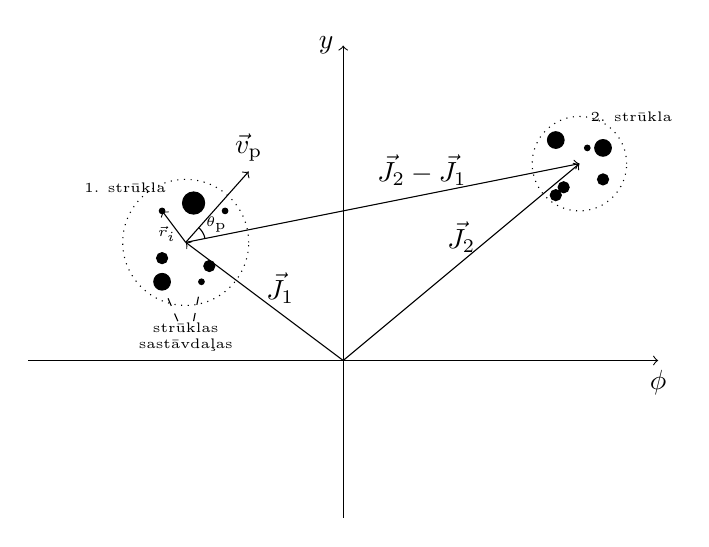
\begin{tikzpicture}
  \coordinate [label=below:$\phi$] (xpos) at (4.0, 0.0);
  \coordinate [label=left:$y$] (ypos) at (0.0, 4.0);
  
  \coordinate (O) at (0.0, 0.0);
  \coordinate (xneg) at (-4.0, 0.0);
  \coordinate (yneg) at (0.0, -2.0);
  \draw[->] (xneg) -- (xpos);
  \draw[->] (yneg) -- (ypos);
  \coordinate (jet1) at (-2.0, 1.5);
  \draw[dotted] (jet1) circle (0.8); 

  \draw[fill=black] (jet1) + (0.5, 0.4) circle (1pt); 
  \draw[fill=black] (jet1) + (-0.3, 0.4) circle (1pt);
  \draw[->](jet1)--($(jet1) + (-0.3, 0.4)$)  node[pos=0.8, below, font=\tiny]{$\vec{r}_{i}$};
  \draw[fill=black] (jet1) + (-0.3, -0.5) circle (3pt); 
  \draw[fill=black] (jet1) + (0.1, 0.5) circle (4pt); 
  \draw[fill=black] (jet1) + (-0.3, -0.2) circle (2pt); 
  \draw[fill=black] (jet1) + (0.3, -0.3) circle (2pt); 
  \draw[fill=black] (jet1) + (0.2, -0.5) circle (1pt); 

  
  \coordinate (jet2) at (3.0, 2.5);
  \draw[dotted] (jet2) circle (0.6); 

  \draw[fill=black] (jet2) + (0.1, 0.2) circle (1pt); 
  \draw[fill=black] (jet2) + (-0.3, 0.3) circle (3pt); 
  \draw[fill=black] (jet2) + (-0.3, -0.4) circle (2pt); 
  \draw[fill=black] (jet2) + (0.3, 0.2) circle (3pt); 
  \draw[fill=black] (jet2) + (-0.2, -0.3) circle (2pt); 
  \draw[fill=black] (jet2) + (0.3, -0.2) circle (2pt); 

  \draw[->](O)--(jet1) node[pos=0.4, above]{$\vec{J}_{1}$}; 
  \draw[->](O)--(jet2) node[midway, above]{$\vec{J}_{2}$}; 
  \draw[->](jet1)--(jet2) node[pos=0.6, above]{$\vec{J}_{2}-\vec{J}_{1}$}; 
  \draw[->](jet1)--($(jet1) + (0.8, 0.9)$) node[at end, above]{$\vec{v}_{\text{p}}$}; 
  \coordinate (vp) at ($(jet1) + (0.8, 0.9)$);
  \draw   pic [draw, angle radius=2.5mm, angle eccentricity=1.8,"$\theta_{\text{p}}$" font=\tiny] {angle=jet2--jet1--vp};
    \node(text) at ($(jet1) + 0.7*(-1.1, 1.0)$) {\fontsize{5}{5}\selectfont 1. strūkla};
    \node(text) at ($(jet2) + 0.6*(1.1, 1.0)$) {\fontsize{5}{5}\selectfont 2. strūkla};
    \node[align=flush center, text width=1.5cm, font=\tiny](text) at (-2.0, 0.3) { strūklas \\  sastāvdaļas};
    \draw[dashed](-2.1, 0.5) -- (-2.25, 0.85);
    \draw[dashed](-1.9, 0.5) -- (-1.82, 0.9);
  
  %\node(text) at (1.1, 1.0) {\fontsiz11e{5}{5}\selectfont$\text{supravadītspēja}$};
  %\node[align=center](text) at (1.5, 3.0) {\fontsize{5}{5}\selectfont normāla \\ \fontsize{5}{5}\selectfont vadītspēja};

  %\node[point] at (A) {};111
  %\node[point] at (B) {};
  %\node[point] at (C) {};

\end{tikzpicture}
\end{document}
